\chapter{AlloSat un corpus pour la reconnaissance continue d'émotions}
\label{chapitre4}
«Vos clients les plus mécontents sont votre meilleure source d’apprentissage»  (Bill Gates, 1955-)

\section{Motivation}
L'un des objectifs de cette thèse est de reconnaître l'état émotionnel de personnes en relation téléphonique avec des agents de centres d'appels. Les motivations de ces conversations sont diverses, mais en général elles concernent soit l'achat d'un produit (service d'abonnement, service d'achat), soit la recherche d'une solution à un problème donné (plainte, service après vente, service de réclamation), soit la demande d'informations diverses sur une entreprise ou leurs produits. Selon l'exigence industrielle, les émotions sont primordiales dans la relation clientèle~\cite{Tumbat2011} :
\begin{itemize}
  \item la satisfaction notamment est un facteur de fidélité et de diffusion de la marque (un client satisfait peut à son tour promouvoir la marque à son entourage),
  \item la frustration favorise l'attrition du client, c'est-à-dire le rejet de la marque au profit de ses concurrents, et la \textit{mauvaise publicité}.
\end{itemize}
Ces deux émotions, comme nous avons pu le voir dans le chapitre~\ref{chapitre1}, peuvent s'inscrire dans différentes théories discrètes ou continues. Pour rappel, il s'agit de deux émotions qui peuvent s'inscrire dans le circumplex de Russell~\cite{Russell1980} (cf Figure 1.6), la satisfaction étant polarisée de façon positive avec une activation plutôt neutre et la frustration étant polarisée de façon plutôt négative, avec une activation assez forte.

En accord avec les besoins de l'entreprise Allo-Média, partenaire de cette thèse, nous avons choisi de les inscrire dans un espace continu, en créant la dimension de satisfaction comme explicitée dans la figure~\ref{fig:satisfactionAxis}. En effet, en plus de la catégorie de l'émotion, la variation de son intensité et de sa durée, permettent de visualiser une dynamique des émotions. Celle-ci est un indicateur crucial pour améliorer l'expérience du client. De plus, Allo-Média, notre partenaire industriel, cherche à définir une satisfaction et une frustration en synchrone. C'est-à-dire que l'entreprise souhaite pouvoir afficher à la fois la catégorie et l'intensité de l'émotion au fur et à mesure de la conversation. Tandis que des émotions discrètes ne contiennent pas autant d'informations. Il est donc plus logique de nous inscrire dans une théorie émotionnelle continue.

\begin{figure}[h]
  \centering
  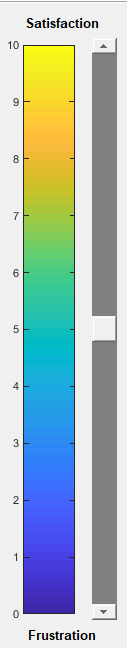
\includegraphics[width=\textwidth]{./Chapitre4/figures/satisfactionAxis.png}
  \caption{L'axe de satisfaction va de la frustration à la satisfaction, en passant par le neutre. C'est donc sur cet axe que l'annotation a été effectuée.}
  \label{fig:satisfactionAxis}
\end{figure}


Pour étudier ces émotions dans ce contexte, nous avons besoin de données et donc d'un corpus. Nos contraintes sont les suivantes :
\begin{itemize}
  \item les conversations doivent provenir de conversations téléphoniques. Elles doivent être assimilables à une relation clientèle où un utilisateur recherche des informations auprès d'un conseiller,
  \item les conversations doivent être en français,
  \item une séparation entre le canal de l'appelant et de l'appelé est souhaitable, pour ne pas avoir de problèmes de chevauchements et donc permettre l'annotation d'un seul locuteur sans être influencé par l'autre locuteur,
  \item l'annotation doit être faite selon l'axe de satisfaction et de frustration. Elle doit également être continue.
\end{itemize}

Nous avons recherché un corpus dans la littérature, notamment parmi ceux décrits dans le chapitre~\ref{chapitre3}, qui répond à toutes ces contraintes. Malheureusement aucun ne correspond parfaitement à notre demande, d'autant plus que peu de corpus comportant des conversations réelles issues de centre d'appel sont disponibles pour la recherche. Nous avons donc décidé de construire un corpus adapté à nos besoins.

\section{Recueil des données}
Avec l'entreprise Allo-Média, nous avons pu recueillir des données provenant de différents centre d'appels français, sous la forme de conversations impliquant des appelants (les clients) et des agents. Comme nous ne voulons pas nous restreindre dans un domaine d'activité donné, nous avons récupéré une cinquantaine de conversations de chaques domaines d'activité des entreprises. Parmi eux, nous avons sélectionné des conversations issues des domaines de l'assurance, de la distribution d'énergie, des agences de voyages, des agences immobilières et de la téléphonie. Ces appels ont eu lieu entre juillet 2017 et novembre 2018.

Ces conversations étant séparées dans l'enregistrement entre le canal du client et le canal de l'agent, nous n'avons donc pas de chevauchement, des \textit{overlaps}, de signal entre les locuteurs. De plus, pour des contraintes éthiques et commerciales, la partie concernant l'agent ne peut être diffusée et a donc été supprimée des données collectées. En effet, Allo-Média ne s'inscrit pas dans une logique de contrôle et de notation des agents. La partie du client quant à elle, est principalement constituée d'un locuteur unique qui ne sera pas retrouvé dans d'autres conversations. Ici, nous avons fait le choix d'étudier les émotions d'un ensemble de locuteurs, plutôt que des émotions d'un seul locuteur : on considère la reconnaissance d'émotion comme indépendante du locuteur. Toutefois, il existe également des conversations où il peut y avoir plusieurs locuteurs, comme par exemple quand une personne passe le téléphone à un autre membre de sa famille. Tous les enregistrements sont issus du canal téléphonique, échantillonné à 8kHz.

Face à cette masse de données, et conscients que nous ne pouvons pas tout annoter, nous avons du mettre en place un processus pour sélectionner les données qui constitueront le corpus.

\subsection{Sélection des données}
Il est communément admis que toute parole n'est pas forcément marqué par des états émotionnels, d'où la présence d'un état neutre. C'est d'autant plus vrai pour des conversations issues de centre d'appels. En effet, lors d'un appel pour une précision sur la livraison d'un produit ou sur le suivi d'un abonnement par exemple, il est rare que des émotions soient exprimées.

A priori la frustration peut se reconnaître par une modification du timbre, une parole plus rapide et des hésitations plus importantes. On peut également noter l'augmentation de la présence du discours para-linguistique avec des soupirs, des bruits de bouches ou des rires nerveux pour la frustration. Le discours se teinte également de mots à polarité négative et présente des répétitions. Dans certains cas, on peut observer une augmentation des tournures négatives. Pour la satisfaction, on assiste à un phénomène inverse, avec une parole moins rapide et plus posée. Le discours se teinte de mots à polarité positive et présente moins de répétitions et moins de prise de parole longue.

En se basant sur ces observations, afin de réduire le coût d'annotation, nous avons donc choisi de sélectionner automatiquement des conversations où la présence de la satisfaction ou de la frustration peut être détectée par l'humain. Pour ce faire, nous avons mis en place plusieurs critères :
\begin{itemize}
  \item La durée de la conversation : celle-ci doit être d'au moins 30 secondes, pour avoir le temps d'exprimer une émotion et pour éviter les appels ratés ou manqués. Comme la frustration et la satisfaction semble être induite par une interaction avec l'agent, nous ne conservons que les conversations composées d'au moins trois tours de parole, soit trois prises de parole de la part du client et du conseiller.
  \item Une forte variation de la fréquence fondamentale. En effet, comme nous l'avons vu précédemment dans le troisième chapitre, la variation de la fréquence fondamentale est une indication permettant de caractériser la prosodie de la parole. Afin d'extraire la fréquence fondamentale, nous avons utilisé l'algorithme appelé Yet Another Algorithm for Pitch Tracking (YAPPT)~\cite{Zahorian2008} qui permet de pallier le contexte téléphonique. En effet, le signal téléphonique possédant une bande passante limitée, la fréquence fondamentale peut en être absente. Cet algorithme cherche donc à restaurer la fréquence fondamentale des signaux dégradés.
  \item La conversation doit être polarisée : pour ce faire, nous avons calculé un score de polarité en partant des transcriptions de la partie du client. En utilisant le dictionnaire French Affective Norms (FAN)~\cite{Monnier2014} que nous avons présenté dans le troisième chapitre, nous avons calculé un score de valence correspondant à la moyenne des scores de chaque mot polarisé présent dans la transcription. Les autres mots sont pris en compte avec le score de 5, considéré comme le neutre. Ce score de valence de la conversation varie donc entre 0 et 10, 0 étant le plus négatif et 10 le plus positif.

  Prenons la phrase \textit{c' est une supercherie, votre cupidité est sans limite} : les termes supercherie et cupidité ont des scores respectivement de $3.32$ et $3.35$. Les autres mots n'ont pas de scores de polarité. Cette phrase a un score de $\frac{3.32+3.35+6\times5}{8}=4.58$.
\end{itemize}

\begin{figure}[h]
  \centering
  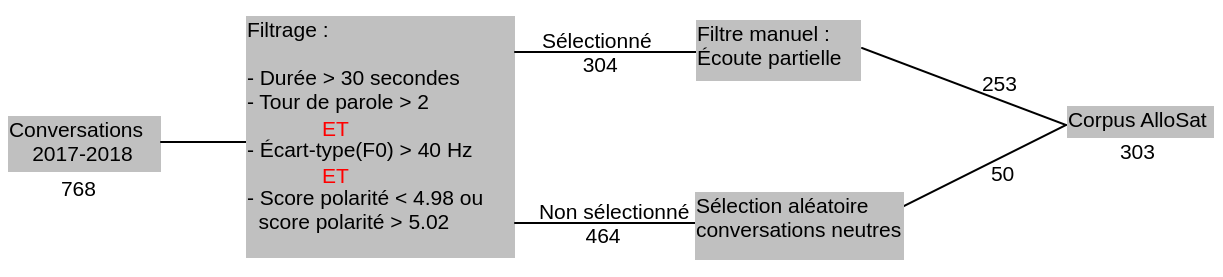
\includegraphics[width=\textwidth]{./Chapitre4/figures/diagchoix.png}
  \caption{Diagramme représentant la chaine de traitement pour la sélection des conversations présentes dans le corpus AlloSat.}
  \label{fig:diagchoix}
\end{figure}


L'application de ces critères a permis d'isoler 304 conversations présentant des caractéristiques intéressantes sur un total de 768 conversations. On peut voir sur le diagramme~\ref{fig:diagchoix} les différents filtres qui ont été appliqués aux conversations. Elles sont d'une durée suffisante, ont un écart type de leurs fréquences fondamentales supérieures à 40 Hz et un score de polarité non compris entre $4.98$ et $5.02$. Ces scores sont très resserrés de par la part importante de mots neutres. Ces 304 conversations ont été écoutées afin de garder les conversations où la manifestation de la dimension de satisfaction était la plus flagrante. Par ce procédé, nous avons conservé 253 conversations.
Afin de mieux respecter la répartition des états émotionnels dans un contexte de centres d'appels, nous avons également sélectionné au hasard 50 conversations qui n'étaient pas retenues par le filtre mis en place et donc considérées comme neutre.

Nous avons donc une sélection finale contenant 303 conversations.
Une fois cette sélection effectuée, nous avons dû traiter les données pour qu'elles puissent être annotées par la suite.

\subsection{Pre-traitement des données}
Les données en l'état ne peuvent pas être immédiatement annotées, des pré-traitements sont nécessaires : la réduction des silences et l'anonymisation des données personnelles.

\subsubsection{Réduction des silences}
Comme les deux canaux (client et agent) sont séparés en amont, nous avons conservé uniquement les documents provenant du canal client, afin de ne pas traiter la parole de l'agent.
L'absence de la réponse du conseiller ajoute de longs moments de silence dans le signal audio. Afin de réduire l'effort d'annotation, nous avons décidé de réduire les silences de plus de deux secondes. Cette réduction suit le protocole suivant :
\begin{itemize}
  \item Nous détectons les silences automatiquement en utilisant l'outil \textit{silencedetect} de ffmepg~\cite{Tomar2006}. Cet outil détecte les zones de conversation dont le volume est inférieur à un seuil de tolérance donné, dans notre cas -40dB, pendant une durée donnée, dans notre cas deux secondes. Ce seuil a été déterminé empiriquement, pour supprimer les silences et quelques bruits parasites, sans détruire des séquences de parole. On liste ainsi les silences qui sont présents dans le document.
  \item On supprime le signal audio dès lors que l'on trouve un silence d'une durée supérieure à deux secondes, en suivant la liste établie précédemment. Si le silence dure moins de deux secondes, on ne le supprime pas.
  \item On réassemble les différents fragments du signal, en intercalant un signal audio de bruit blanc d'une durée exacte de deux secondes. Un bruit blanc correspond à une génération automatique d'un signal audio par le tirage aléatoire de fréquences suivant la même densité spectrale de puissance. Dans notre cas, nous avons crée un bruit blanc en suivant la loi normale. Ce choix a été motivé par une volonté de confort pour les annotateurs.
\end{itemize}

\begin{figure}[h]
  \centering
  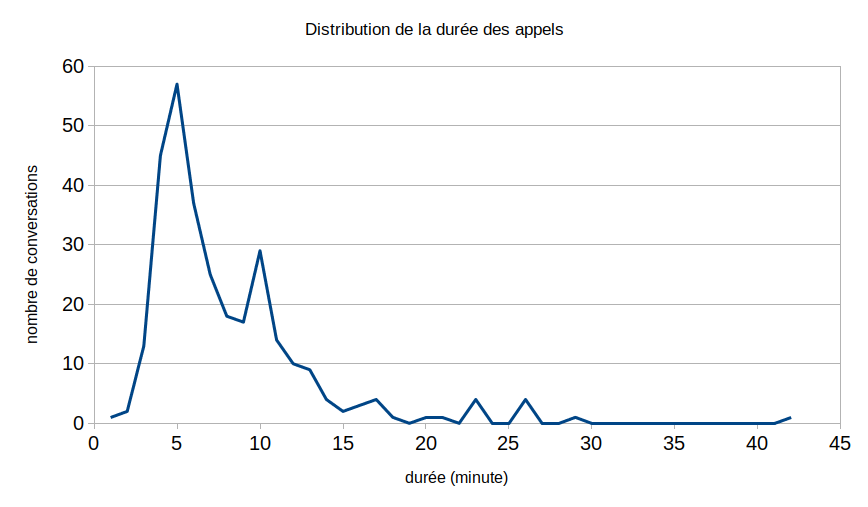
\includegraphics[width=15cm]{./Chapitre4/figures/repart.png}
  \caption{La répartition des conversations en fonction de leur durée. En bleu, nous avons les anciennes durées, en orange les nouvelles. Environ $76,6\%$ des conversations duraient moins de 15 minutes (soit 900 secondes). Après réduction des silences, ce nombre augmente à environ $93,7\%$.}
  \label{fig:repart}
\end{figure}


Ce traitement nous permet de passer d'un corpus de 57 heures majoritairement composé de silences à un corpus de 37 heures où les silences sont contrôlés. Nous avons donc une répartition des durées de conversation plus homogènes, comme le montre la figure~\ref{fig:repart}. Les conversations ont une durée variant de 32 secondes à 41 minutes, avec une moyenne d'environ 7 minutes.

Une fois ce traitement effectué, nous avons mis en place l'anonymisation du corpus.

\subsubsection{Anonymiser les données personnelles}

\begin{table}[h]
    \centering
\begin{forest}
  for tree={grow'=east, anchor=west}
  [Données personnelles
    [personne
      [prenom
        [épellation]
      ]
      [nom
        [épellation]
      ]
      [mail]
      [date de naissance]
    ]
    [numéro
      [téléphone]
      [carte bancaire]
      [RIB]
      [INSEE]
      [immatriculation]
    ]
    [localisation
      [ville]
      [voirie]
      [code postal]
    ]
    [autre
      [marque]
      [produit]
    ]
  ]
\end{forest}
\label{tab:donneesPerso}
\caption{Arbre des différentes catégories de données personnelles anonymisées}
\end{table}


Afin de respecter la vie privée des personnes, la France et les autres pays européens ont mis en place une réglementation sur la collecte, le stockage et le traitement des données personnelles de tout individu. Le règlement général sur la protection des données (RGPD) établit des règles relatives à la protection des utilisateurs vis à vis du traitement de leur données personnelles, pour s'assurer que les utilisateurs conservent leurs libertés et leurs droits fondamentaux. Cette réglementation, contrôlée par la Commission Nationale de l'Informatique et des Libertés (CNIL) a été mise en application en 2018, nous avons donc dû traiter les données du corpus afin de respecter cette réglementation.

Un des points les plus importants de cette réglementation est l'obfuscation de toutes les données personnelles. Les catégories de données personnelles que nous avons anonymisées sont présentées dans l'arbre~\ref{tab:donneesPerso}. Ce sont celles définies par l'entreprise Allo-Média, en accord avec les réglementations en vigueur. Il est à noter que l'anonymisation ne se fait pas exclusivement par les feuilles de l'arbre, tous les nœuds peuvent être utilisés. L'anonymisation des nœuds est exceptionnelle, elle obstrue les données indirectes qui permettent de reconnaître un individu. Par exemple, dans le cadre de la localisation, un nom donné à une maison \textit{l'hirondelle} est anonymisé en catégorie \textit{localisation}. À ces dernières s'ajoutent aussi les données permettant d'identifier des entreprises. Les marques et les produits sont obfusqués. Ainsi, les conversations finales permettent de reconnaître le domaine d'activité de l'entreprise mais pas son identité.

\begin{figure}[h]
  \centering
  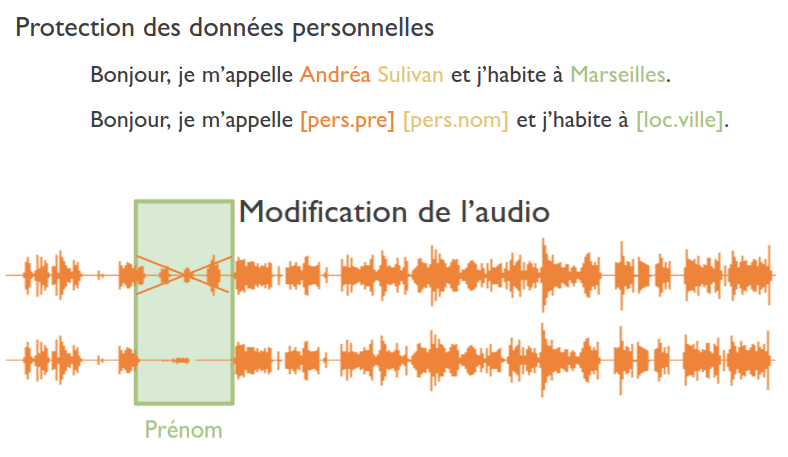
\includegraphics[width=15cm]{./Chapitre4/figures/annony.png}
  \caption{Exemple d'obfuscation d'un segment fictif. Les mots sont d'abord retrouvés dans la transcription, puis sont substitués par leur catégorie. Enfin le signal audio est modifié pour remplacer les informations personnelles par un son pré-enregistré.}
  \label{fig:annony}
\end{figure}


Pour procéder à cette obfuscation, nous avons utilisé un obfuscateur automatique, détenu par la société Allo-Média, appliqué sur les transcriptions, puis répercuté sur les fichiers audio. Ce parseur, dans un premier temps, recherche les mots appartenant aux groupes présentés dans l'arbre~\ref{tab:donneesPerso}, dans les transcriptions des conversations. Il substitue dans le texte les mots désignés par la catégorie. Enfin il substitue le segment audio correspondant au code temporel des données personnelles détectées par un signal audio pré-enregistré. Ce dernier se compose d'un air de percussion de type jazzy. Un exemple fictif de cette obfuscation est illustré dans la figure~\ref{fig:annony}.

Une deuxième passe, humaine cette fois ci, permet de garantir l'obfuscation de toutes les données personnelles. En utilisant l'outil Transcriber, chaque conversation a été écoutée et lue, permettant d'identifier et de segmenter les données personnelles restantes. C'est lors de cette deuxième phase que les données permettant d'identifier les entreprises ont été isolées. Nous avons également choisi de supprimer tous les numéros permettant d'identifier un contrat ou une date significative. Les segments identifiés sont alors substitués par le même signal audio jazzy. Ce choix de remplacement est motivé par des retours des annotateurs : nous avons proposé plusieurs sons pour masquer les données personnelles (bruits blancs, son de guitare, de chant, de basse, de percussion...) et ils ont voté pour le moins fatigant.

Lors de cette passe, les annotateurs ont également effectué une correction partielle de la transcription : ils ont eu pour consigne de corriger les segments de parole effectifs, et de ne pas modifier les erreurs de transcription lors que le locuteur ne parle pas au conseiller.
%stats sur les moments d'anonymisation et justifications du sonjazzy

\section{Mise en place de l'annotation}

\subsection{Volonté d'annotation}
%\subsection{Les deux annotations}
Comme nous l'avons dit précédemment, nous souhaitons analyser l'axe de satisfaction de manière continue. Pour cela, nous avons mis en place un axe dont les extrema sont la frustration (0) et la satisfaction (10) qui passe par un état neutre (5) situé à mi-chemin entre ces deux émotions comme montré dans la figure~\ref{fig:satisfactionAxis}. La valeur de satisfaction est automatiquement extraite en continu toutes les 250~ms, ce qui nous permet d'avoir quatre valeurs par seconde. Cette extraction est cohérente avec notre tâche puisque les émotions s'expriment sur un temps long, généralement de l'ordre de la minute~\cite{Schuller2010}.
%Nous avons fait ce choix parce que, contrairement aux mots qui sont analysés dans des fenêtres de 30ms pour la reconnaissance automatique de la parole, les émotions s'expriment sur une période de temps plus longue, généralement de l'ordre de la minute~\cite{Schuller2010}. %Cette annotation étant influencée par l'affect des annotateurs, nous avons cherché des moyens de valider cette annotation entre les différents annotateurs mais aussi par annotateur.

Pour enrichir l'annotation, nous avons décidé de mettre en place, en plus de l'annotation continue, une annotation discrète de la dimension de satisfaction. Cette annotation discrète est effectuée au niveau de la conversation. La catégorie émotionnelle du début et de la fin d'une conversation, comprise entre très frustré, frustré, neutre, satisfait, très satisfait est annotée. La durée de ce début et de cette fin de conversation sont laissées à l'appréciation des annotateurs. En plus, une caractérisation de l'évolution de l'émotion est annotée selon les catégories suivante : montante, descendante, stagnante, varie, varie fortement. Pour mieux comprendre ces catégories, elles ont été explicitées par les schémas de la figure~\ref{fig:variation}, qui ont été montré aux annotateurs.

\begin{figure}
  \centering
  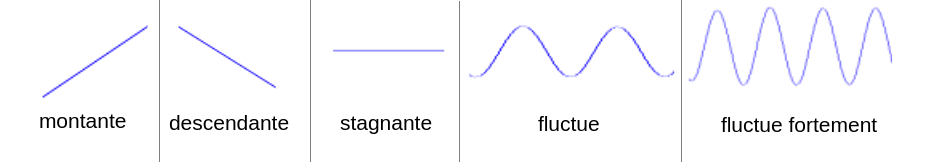
\includegraphics[width=14cm]{./Chapitre4/figures/variation.png}
  \caption{Schéma des variations qui ont été données aux annotateurs afin de mieux comprendre la catégorie évolution}
  \label{fig:variation}
\end{figure}


Afin de comparer AlloSat aux corpus existants, nous avons également mis en place une annotation de la valence sur le même principe que l'annotation discrète de la dimension de la satisfaction. Elle relève la valence de début et de fin de conversation, comprise entre très négative, négative, neutre, positive, très positive. On y ajoute la même caractérisation de l'évolution de la valence. Le tableau~\ref{tab:annotationDiscrete} récapitule les annotations discrètes.

\begin{table}[h]
    \centering
    \begin{tabular}{|p{3cm}|c|}
        \hline
        \multicolumn{2}{|l|}{\textbf{Satisfaction \& Frustration}} \\
        \hline
          debut       & très frustré, frustré, neutre, satisfait, très satisfait \\
          fin         & très frustré, frustré, neutre, satisfait, très satisfait \\
          evolution   & montante, descendante, stagnante, varie, varie fortement \\
         \hline
         \multicolumn{2}{|l|}{\textbf{Valence}} \\
         \hline
         debut        & très négative, négative, neutre, positive, très positive \\
         fin          & très négative, négative, neutre, positive, très positive \\
         evolution    & montante, descendante, stagnante, varie, varie fortement \\
         \hline
    \end{tabular}
    \caption{Récapitulatif du schéma d'annotation discrète.}
    \label{tab:annotationDiscrete}
\end{table}


La différence entre la dimension de satisfaction et la valence a fait l'objet de plusieurs séances d'explication auprès des annotateurs, afin que ces deux notions ne soient pas confondues par les annotateurs.

Pour récapituler, nous nous sommes concentrés sur deux notions :
\begin{itemize}
  \item L'évolution d'une émotion : tous les appels commencent au 'neutre' et évoluent en fonction du temps entre frustration et satisfaction. Cette annotation est continue.
  \item Une évaluation de l'émotion à posteriori : une fois l'appel terminé, nous voulons avoir un retour sur l'évolution de l'émotion. Pour cela nous voulons savoir comment était l'appelant au début de la conversation, comment il était à la fin et comment était cette évolution. Cette annotation est donc discrète.
\end{itemize}

\subsection{Logiciel utilisé}

Nous avons dans un premier temps considéré l'utilisation de FeelTrace~\cite{Cowie2000}, l'outil le plus utilisé pour réaliser de l'annotation continue. Cependant l’outil est optimisé pour annoter deux dimensions à la fois, la valence et l'activation, afin de placer l'annotation dans un contexte bi-dimensionnel qui ne correspond pas avec notre définition de l'axe de satisfaction. De plus, cet outil est assez difficile à prendre en main, et il requiert l'utilisation d'un joystick.

Nous avons donc fait le choix d’utiliser CARMA (Continuous Affect Rating And Media Annotation)~\cite{Girard2014}. CARMA permet d'annoter de façon continue l'émotion selon une dimension définie en amont en utilisant un clavier et une souris. La figure~\ref{fig:carma} montre l'interface visible par les annotateurs lors de l'annotation. Un guide d'installation et de configuration a été fourni à l'administrateur Système de l'entreprise. Il est disponible dans l'annexe~\ref{ap:guideInstall}

\begin{figure}[h]
  \centering
  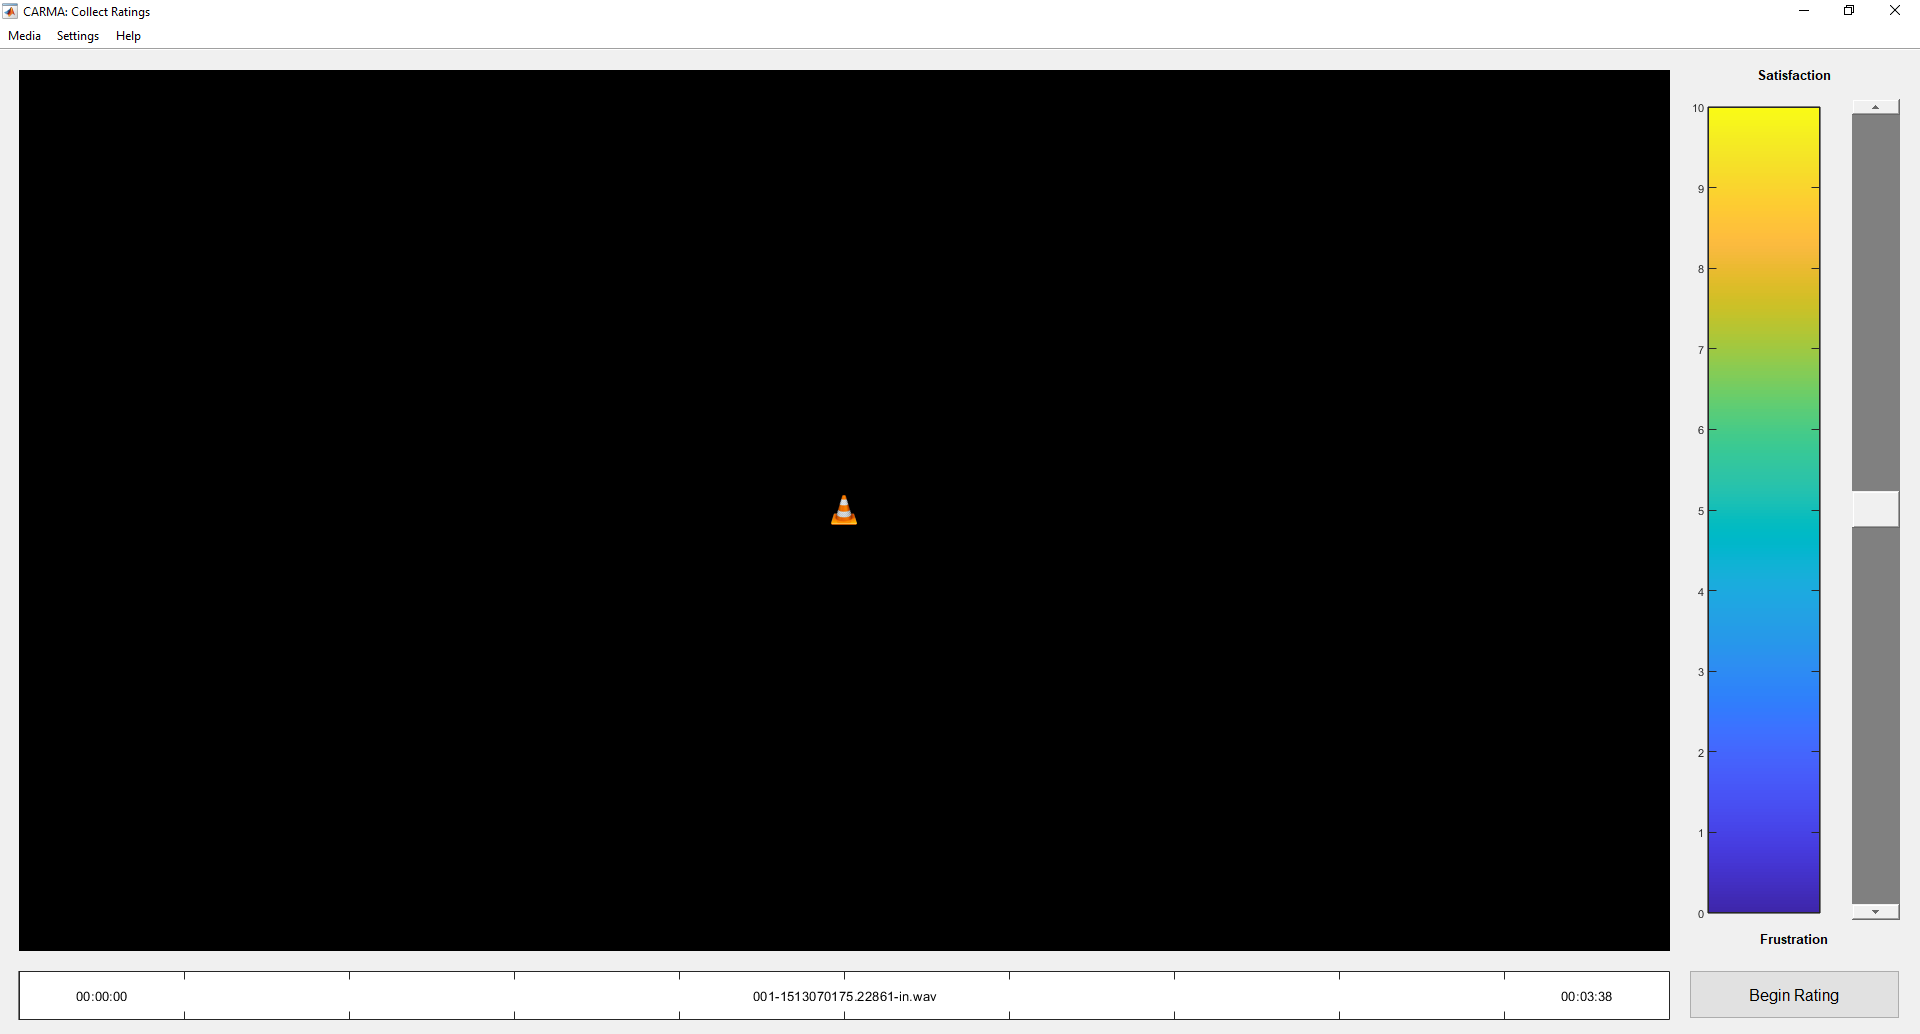
\includegraphics[width=15cm]{./Chapitre4/figures/carma.png}
  \caption{Capture d'écran de l'outils CARMA~\cite{Girard2014}}
  \label{fig:carma}
\end{figure}


Pour l'annotation discrète, les annotateurs ont rempli un modèle pré-construit vide de tableau avec un logiciel bureautique de type Excel. Comme nous l'avons dit précédemment, il y a six catégories à remplir par conversation (état émotionnel de début, de fin et la forme de l'évolution entre les deux). Nous avons également demandé l'annotation en genre des appelants et un espace était mis à disposition pour d'éventuels commentaires.

\subsection{Consignes}

L'annotation a été réalisée par une équipe de trois annotateurs (deux femmes et un homme), employés d'une société de transcription manuelle de la parole basée en France. Ils avaient déjà collaboré avec l'entreprise Allo-Média pour des tâches de transcription manuelle de la parole et d'annotation de données sémantiques, notamment de l'annotation d'entités nommés et des résumés des conversations.

Ces personnes ont donc reçu en amont des formations sur ces différentes tâches : la reconnaissance d'une entité nommée, l'utilisation de l’outil Transcriber, des formations sur l’orthographe et sur la conjugaison notamment.

Afin d'aider les annotateurs et de guider au mieux l'annotation, un guide d'annotation a été mis à leur disposition. Ce guide est disponible dans l'annexe~\ref{ap:guidelines}. Ce dernier explique le contexte de l'étude et les consignes à respecter. Comme l'émotion possède une part non négligeable de subjectivité, il fallait que les consignes soient les plus objectives possibles, tout en assurant l'homogénéité des annotations.

%\begin{itemize}
  %\item Objectivité de l'annotation.
\subsubsection{Objectivité des annotations}
\begin{itemize}
  \item Pour réduire la subjectivité de l'annotation, les annotateurs ne doivent pas prendre parti pour le locuteur durant la conversation.
  \item Les annotateurs ne doivent pas échanger entre eux au sujet des conversations écoutées.
  \item Pour ce qui est des dimensions discrètes, elles doivent être annotées tout de suite après l'écoute de la conversation, afin que les états émotionnels ne soient pas oubliés ou pollués par l'écoute d'autres conversations. De plus le genre des locuteurs et des observations diverses peuvent être rajoutés par les annotateurs.
  \item Chaque conversation est annotée une seule fois par chaque annotateur.
\end{itemize}

\subsubsection{Homogénéité des annotations}
\begin{itemize}
  \item Pour expliquer la notion de valence, nous avons utilisé le Self-Assessment Manikin (SAM)~\cite{Bradley1994} qui donne une description visuelle de la valence, que l'on retrouve sur la figure~\ref{fig:SAM}.
  \item Pour leur permettre d'avoir une meilleure compréhension de la satisfaction et de la frustration que nous voulons annoter, nous avons fourni deux conversations en tant que borne de satisfaction et borne de frustration, afin d'aider à étalonner les émotions. Ainsi les annotateurs peuvent appréhender l'amplitude potentielle de la dimension de satisfaction de façon homogène. Ces bornes ont été établies de façon empirique, lorsque nous avons sélectionné les données du corpus.
\end{itemize}


\begin{figure}
  \centering
  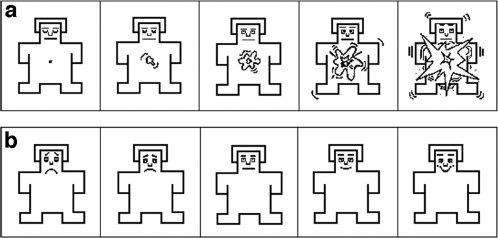
\includegraphics[width=12cm]{./Chapitre4/figures/sam.jpeg}
  \caption{Le Self Assessment Manikin (SAM). La ligne a correspond à l'activation, la ligne b correspond à la valence.}
  \label{fig:SAM}
\end{figure}


%Pour palier à l'aspect subjectif, ils ont été informés que tous les annotateurs annotent les mêmes conversations. Comme l'empathie peut avoir un grand impact sur l'annotation des émotions, nous avons demandé aux annotateurs d'être le plus objectif dans leur annotation et de ne pas prendre parti.

L'annotation de la dimension de satisfaction a donc été réalisée de façon continue selon les consignes suivantes :
\begin{itemize}
  \item La barre d'annotation va de 0 (Frustration) à 10 (Satisfaction), et elle est graduée par palier de 1. Le 5 correspond à l'état neutre et à l'état de départ de l'annotation.
  \item Le curseur d'annotation peut être contrôlé par la souris ou par les flèches du clavier. Les pas du clavier sont de 0.1 tandis que la souris peut avoir une granularité plus fine.
  \item Si aucun état émotionnel n'est constaté, ou qu'il ne varie pas, alors l'annotateur ne doit pas toucher à l'annotation. Cela est valable également lors des silences. Les annotateurs ont été notifiés de la présence de conversations où aucun état émotionnel n'a été constaté en amont.
  \item Un document ne doit être annoté qu'une seule fois par la même personne, sans possibilité de revenir en arrière. Nous voulons la réaction immédiate des annotateurs et non une réaction plus réfléchie, qui tend à minimiser les émotions détectées, selon des travaux préliminaires que nous avons réalisés. Il n'est pas non plus possible d'avancer la conversation, l'annotation doit être faite en temps réel de l'écoute de la conversation.
  \item Un document doit être annoté en une seule fois. On ne doit pas revenir à l'annotation d'un fichier après une longue pause (plusieurs heures ou un jour). Cela évite à l'annotateur de ne plus être dans le contexte émotionnel de la conversation.
\end{itemize}

Ces consignes ont pour but d'aider l'annotateur à effectuer une annotation la plus objective possible. En plus de ces consignes, la structuration des documents a été expliquée. Les bruits blancs indiquent qu'un silence de plus de 2 secondes s'est produit. Les silences ont été retirés du document afin fluidifier l'écoute et l'annotation du document. Ce son est donné à titre informatif pour aider dans l'annotation. Nous avons signalé également la présence de bruits jazzy qui sont utilisés pour l'anonymisation des conversations. Ils remplacent les parties de conversation qui permettent l'identification de personnes ou d'entreprise.

\section{Analyse d'AlloSat}

\begin{table}[]
\begin{tabular}{|l|l|l|l|}
\hline
      & Nombre de conversations & Durée    & Durée de parole \\ \hline
TRAIN & 201                     & 25h26m35 & 15h48m50        \\ \hline
DEV   & 42                      & 05h55m46 & 03h22m14        \\ \hline
TEST  & 60                      & 05h58m41 & 03h28m57        \\ \hline
\end{tabular}
\caption{Découpage du corpus en ensemble de train, développement et test. Les durées sont données en heures, minutes, secondes.}
\label{tab:repartitionEnSets}
\end{table}


AlloSat est composé de 303 conversations, d'une durée totale de 37 heures 23 minutes et 27 secondes, de 308 locuteurs distincts dont 191 femmes et 117 hommes (voir analyse en genres dans le chapitre 7).
%Ces conversations ont été annotées par trois annotateurs, deux femmes et un homme, formés à la transcription d'appels et à l'annotation en catégorie discrètes de concepts sémantiques.
Une répartition semi aléatoire en trois sous-ensembles a été définie. Nous avons veillé à ce que chaque partition comprenne des conversations choisi aléatoirement qui peuvent être dépourvues de contexte émotionnel. L'ensemble d’entraînement (train) est composé de 201 conversations, l'ensemble de développement (dev) de 42 conversations et l'ensemble de test (test) de 60 conversations. De plus amples détails sont disponibles dans le tableau~\ref{tab:repartitionEnSets}.
On peut noter que la durée du dev et du test sont très similaires. On a donc une répartition approximative de 25 heures et demi des données dans le train et douze heures des données dans le dev et le test (avec six heures chacun). Comme nous l'avons vu au chapitre 2, le découpage d'un corpus en sous-ensembles permet d'assurer la cohérence des scores notamment.

% Please add the following required packages to your document preamble:
% \usepackage{multirow}
\begin{table}[]
\begin{tabular}{|l|l|l|l|l|l|l|}
\hline
\multirow{18}{*}{Axe de Satisfaction} & \multicolumn{6}{l|}{Début de la conversation}                                      \\ \cline{2-7}
                                      &                  & neutre & frustré & satisfait & très frustré & très satisfait    \\ \cline{2-7}
                                      & a1               & 300    & 3       & 0         & 0            & 0                 \\ \cline{2-7}
                                      & a2               & 284    & 19      & 0         & 0            & 0                 \\ \cline{2-7}
                                      & a3               & 298    & 5       & 0         & 0            & 0                 \\ \cline{2-7}
                                      & vote majo. & 299    & 4       & 0         & 0            & 0                 \\ \cline{2-7}
                                      & \multicolumn{6}{l|}{Fin de la conversation}                                        \\ \cline{2-7}
                                      &                  & neutre & frustré & satisfait & très frustré & très satisfait    \\ \cline{2-7}
                                      & a1               & 111    & 123     & 21        & 48           & 0                 \\ \cline{2-7}
                                      & a2               & 92     & 91      & 15        & 105          & 0                 \\ \cline{2-7}
                                      & a3               & 56     & 48      & 53        & 135          & 11                \\ \cline{2-7}
                                      & vote majo. & 85     & 195     & 23        & 0            & 0                 \\ \cline{2-7}
                                      & \multicolumn{6}{l|}{évolution}                                                     \\ \cline{2-7}
                                      &                  & stagne & descend & monte     & fluctue      & fluctue fort \\ \cline{2-7}
                                      & a1               & 87     & 165     & 10        & 39           & 2                 \\ \cline{2-7}
                                      & a2               & 50     & 193     & 8         & 51           & 1                 \\ \cline{2-7}
                                      & a3               & 64     & 193     & 19        & 27           & 0                 \\ \cline{2-7}
                                      & vote majo. & 55     & 184     & 7         & 57           & 0                 \\ \hline \hline
\multirow{18}{*}{Valence}             & \multicolumn{6}{l|}{Début de la conversation}                                      \\ \cline{2-7}
                                      &                  & neutre & négatif & positif   & très négatif & très positif      \\ \cline{2-7}
                                      & a1               & 298    & 5       & 0         & 0            & 0                 \\ \cline{2-7}
                                      & a2               & 280    & 22      & 1         & 0            & 0                 \\ \cline{2-7}
                                      & a3               & 298    & 5       & 0         & 0            & 0                 \\ \cline{2-7}
                                      & vote majo. & 299    & 4       & 0         & 0            & 0                 \\ \cline{2-7}
                                      & \multicolumn{6}{l|}{Fin de la conversation}                                        \\ \cline{2-7}
                                      &                  & neutre & négatif & positif   & très négatif & très positif      \\ \cline{2-7}
                                      & a1               & 93     & 136     & 19        & 55           & 0                 \\ \cline{2-7}
                                      & a2               & 86     & 105     & 20        & 92           & 0                 \\ \cline{2-7}
                                      & a3               & 55     & 50      & 53        & 135          & 10                \\ \cline{2-7}
                                      & vote majo. & 91     & 188     & 24        & 0            & 0                 \\ \cline{2-7}
                                      & \multicolumn{6}{l|}{évolution}                                                     \\ \cline{2-7}
                                      &                  & stagne & descend & monte     & fluctue      & fluctue fort \\ \cline{2-7}
                                      & a1               & 89     & 164     & 8         & 40           & 2                 \\ \cline{2-7}
                                      & a2               & 44     & 185     & 14        & 57           & 3                 \\ \cline{2-7}
                                      & a3               & 56     & 196     & 22        & 29           & 0                 \\ \cline{2-7}
                                      & vote major. & 52     & 184     & 8         & 59           & 0                 \\ \hline
\end{tabular}
\label{tab:statistiqueAnnotation}
\caption{Ensemble des annotations discrètes des trois annotateurs a1, a2 et a3. Vote majo correspond au vote majoritaire qui a conduit à l'annotation discrète de référence}
\end{table}


Le tableau~\ref{tab:statistiqueAnnotation} regroupe l'ensemble des annotations discrètes du corpus. Nous pouvons observer une sur-représentation de l'état neutre, surtout en début de conversation, ce qui ne nous a pas surpris, puisque l'on retrouve peu de passage marqué par un état émotionnel dans la parole. Comme nous le pensions, la plupart des conversations ont été perçues avec une frustration croissante, probablement parce que la plupart des clients appelle quand ils ont un problème ou par exemple parce que le conseiller n’est pas en mesure de donner une réponse suffisamment satisfaisante à l’interlocuteur.

Comme nous pouvons le voir dans le tableau~\ref{tab:statistiqueAnnotation}, peu de conversations ont été annotées en très satisfait. Nous avons donc choisi de regrouper les catégories très satisfaites et satisfaites. Afin de rester symétrique dans nos annotations, nous avons également regroupé les catégories très frustrées et frustrées. Les annotations discrètes sont ensuite fusionnées par vote majoritaire. En cas d'égalité,
%Si nous avons les trois catégories pour une observation en début et fin de conversation,
nous choisissons le neutre que ce soit pour la valence ou la dimension de satisfaction. Pour l'évolution des deux axes, le vote majoritaire n'est pas suffisant pour fusionner les données : il y a trop de cas d'égalité. Nous avons considéré que si l'évolution était différentes selon les annotateurs, elle correspond à la catégorie \textit{fluctue}.

%Afin d'évaluer la pertinence du corpus, nous avons étudiés l'annotation de ces trois annotateurs.
Nous avons mis en place des mesures d'accord intra-annotateurs, permettant de mesurer la pertinence d'une annotation vis à vis des autres annotations du même annotateur. Et nous avons également mis en place des mesures d'accord inter-annotateurs, permettant de mesure la pertinence de l'annotation d'un document par rapport à une autre annotation du même document. %Ainsi, nous avons des informations sur la difficulté de la tâche et sur le niveau de subjectivité des annotateurs notamment.

\subsection{Accord intra-annotateur}

Cet accord est mesuré entre les annotations continues et discrètes d'une même conversation par un même annotateur. Les annotations continues ont été normalisées en suivant la méthode de la normalisation standard selon l'équation~\ref{eq:normStand} avec une annotation $x$ issue de toutes les annotations $X$, remettant les annotations dans un espace allant de zéro à un.

\begin{equation}
  x' = \frac{x-Minimum(X)}{Maximum(X)-Minimum(X)}
  \label{eq:normStand}
\end{equation}

Nous avons discrétisé les valeurs continues, appelée $S_n$ dans la suite, suivant les trois niveaux utilisés dans l'annotation discrète. Pour ce faire, nous avons défini empiriquement deux seuils en observant l'annotation des conversations neutres contenues dans le corpus. En effet, l'annotation de ces dernières restent globalement entre les bornes 0.45 et 0.55 de l'axe de satisfaction. Notre seuil permet de déterminer si une valeur continue correspond à un état de frustration ($S_n<0.45$), à un état neutre ($0.45 < S_n < 0.55$) ou à un état de satisfaction ($S_n > 0.55$).

Nous avons également défini la notion de début et fin de conversation comme étant $10\%$ de la durée de la conversation, $dc$.
%Ensuite nous avons défini les notions de début et fin de conversation dans le contexte de l'annotation continue. Nous avons déterminé qu'il était chacun constitué de 10\% de la durée totale de la conversation, appelé $dc$.
Le début correspond donc au segment commençant à 0 et finissant à $0.1\times dc$ et la fin correspond au segment commençant à $ dc - 0.1\times dc$ , jusqu'à la fin de la conversation, $dc$.

Nous avons alors fait la moyenne des valeurs de satisfaction sur le début de la conversation et nous appliquons le seuillage pour déterminer quelle étiquette caractérise cet intervalle de temps. Nous faisons exactement la même chose avec les annotations de fin de conversation. Ainsi pour chaque conversation, nous avons l'annotation discrète effectuée par l'annotateur et une autre annotation discrète correspondant à la discrétisation de son annotation continue.
La différence entre l'annotation discrétisée du début et de la fin de la conversation devrait être en adéquation avec l'évolution annotée.

Nous avons également décidé de calculer un kappa par annotateur.
Le kappa ($\kappa$) est une mesure permettant de quantifier l'accord entre deux observations. Elle mesure le degré de concordance entre deux observations selon l'équation~\ref{eq:kappa}:
\begin{equation}
    \kappa = \dfrac{P_0 - P_e}{1 - P_e}
    \label{eq:kappa}
\end{equation}

$P_0$ correspond à l'accord relatif des observations entre les annotations et $P_e$ représente la probabilité d'un accord aléatoire. Comme nous avons un cas de sur-représentation d'une classe, ici le neutre, nous avons fixé $P_e$ à $1/3$ suivant les recommandations de Callejas et al.~\cite{Callejas2008}.

Le kappa est compris entre 0 et 1. Plus le kappa est proche de 1, plus l'accord entre les deux observations est forte. En revanche, plus le kappa se rapproche de 0 et moins on a d'accord entre les observations. De plus, le kappa permet d'indiquer la difficulté de la tâche à effectuer, dans le cas d'une tâche subjective comme la nôtre. Généralement, on considère le kappa comme suffisant lorsqu'il est proche de 0.8. D'après McHugh~\cite{McHugh2012}, si on rapproche le kappa à l'accuracy, un coefficient de 0.8 correspond à environ 64\% d'accuracy, étant qualifié d'accord fort.

\begin{table}[th]
  \centering
  \begin{tabular}{|p{2cm}| l l | l l|}
    \hline
        &\multicolumn{2}{c}{\textbf{Nombre de désaccord}} & \multicolumn{2}{c}{\textbf{kappa}} \\
              &début  &fin    &début      &fin  \\
    \hline
    a1        &4      &31     &0.98       &0.84	\\
    a2        &23     &55     &0.88       &0.72 \\
    a3        &13     &50     &0.93       &0.75	\\
    \hline
    Moyenne  &13.33 &45.33 &0.93   &0.77 \\
    \hline
  \end{tabular}
\caption{Nombre de désaccord et kappa pour définir l'accord intra-annotateur pour chacun des trois annotateurs ainsi que la moyenne. $a_i$ represente l'annotateur $i$.}
\label{tab:accordIntraAnnot}
\end{table}

Les résultats de ces calculs sont disponibles dans le tableau~\ref{tab:accordIntraAnnot}. Nous pouvons observer une forte concordance entre les annotations discrètes et les annotations continues discrétisées dans les débuts de conversation avec un kappa moyen de 0.93. Si on se concentre sur le nombre de cas où l'annotation discrète est différente de l'annotation continue discrétisée, on voit que le premier annotateur (a1) a environ 1\% de désaccord et qu'au maximum, l'annotateur 2 (a2) est en désaccord de moins de 8\%.
Pour les fins de conversation, on observe de moins bons scores, avec un kappa moyen de 0.77 mais qui reste suffisant pour exprimer une cohérence des annotations. En regardant le nombre d'annotations différentes, on observe de nouveau que l'annotateur 1 (a1) a le moins de désaccord avec moins de 10\%, tandis que l'annotateur 2 (a2) culmine à presque 17\% de désaccord.
Nous avons conclu que, même si l'accord intra-annotateur n'est pas parfait, il est suffisant pour certifier de la cohérence des annotations continues et discrètes produites par un même annotateur.

\subsection{Accord inter-annotateur}
Afin d’évaluer l’accord inter-annotateur sur les annotations continues, nous avons utilisé le coefficient de corrélation linéaire. Ce coefficient est calculé au niveau de la conversation sur la dimension de satisfaction normalisée par rapport à l’ensemble des conversations entre les paires d’annotateurs comme défini dans la section précédente.

Le coefficient de corrélation linéaire donne une mesure de l'intensité et du sens de la relation linéaire entre deux variables, ici les deux annotations des deux annotateurs. Son calcul est défini par l'équation suivante~\ref{eq:coeffCorr}:
\begin{equation}
  R_{12} = \dfrac{Cov(x_1,x_2)}{\sigma_{x_1}*\sigma_{x_2}}
  \label{eq:coeffCorr}
\end{equation}
où $Cov(x_1,x_2)$ désigne la covariance entre les variables $x_1$ et $x_2$, ici l'ensemble des annotations de deux annotateurs $a_1$ et $a_2$. $\sigma_{x_1}$, $\sigma_{x_2}$ désignent leur écart type.
Ce coefficient est compris entre -1 et 1. Plus il est proche de 1, plus la relation linéaire positive entre les variables est forte. Plus il est proche de -1, plus la relation linéaire négative entre les variables est forte. Si le coefficient est proche de 0, on ne peut pas établir de relation linéaire.
Nous avons également calculé le kappa entre paires d'annotateur sur les valeurs discrètes de début et de fin de conversation.

\begin{table}[th]
    \centering
    \begin{tabular}{| p{1cm} | l | l l |}
    \hline
      & \multicolumn{1}{c|}{$R$} & \multicolumn{1}{c}{$\kappa^{début}$} & \multicolumn{1}{c}{$\kappa^{fin}$}\\
      \hline
      a1-a2   &0.82   &0.99   &0.90   \\
      a2-a3   &0.87   &0.88   &0.69   \\
      a1-a3   &0.80   &0.87   &0.72   \\
      \hline
      Moyenne &0.83   &0.91   &0.77   \\
      \hline
    \end{tabular}
    \caption{Accord inter-annotateur calculé entre les pairs d'annotateurs ainsi que la moyenne.$a_i$ représente l'annotateur $i$. $R$ represente le coefficient de corrélation, \kappa représente le kappa de début et de fin de conversation.}
    \label{tab:accordInterAnnot}
  \end{table}


Les valeurs rapportées dans le tableau~\ref{tab:accordInterAnnot} montrent une bonne corrélation entre les annotateurs (un coefficient de corrélation moyen de 0,83), ce qui signifie que les annotations continues sont cohérentes entre les annotateurs.
On observe toutefois que l'annotateur 1 (a1) et l'annotateur 3 (a3) sont moins enclin à donner les mêmes annotations que les paires d'annotateurs a1-a2 et a2-a3.

On remarque également que le kappa de début de conversation est très élevé. L’une des raisons de ce fort accord est que le début de la conversation est presque toujours neutre. Cela peut s’expliquer de deux façons. Tout d’abord, l’annotation continue est toujours initialisée à cinq, ce qui se traduit par un état neutre. Nous avons donc un biais introduit par cet état initial, qui permet à toutes les annotations de commencer de la même manière.
Mais l’hypothèse principale est que l’interlocuteur est rarement frustré ou satisfait en début de l’appel : ces émotions sont provoquées par les réponses de l’agent.

\begin{figure}[h]
  \centering
  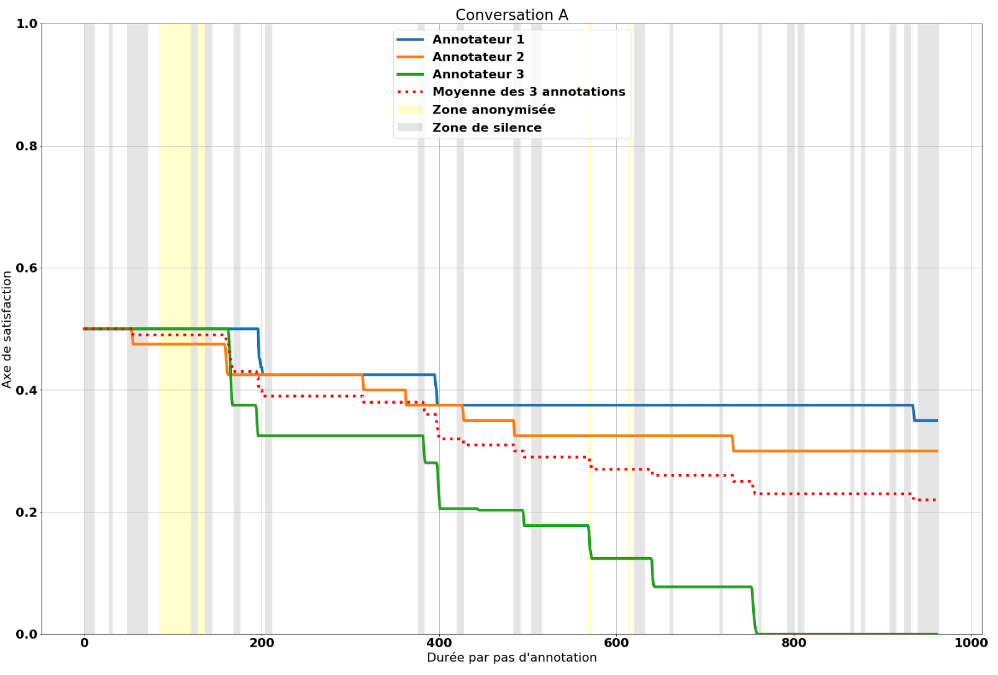
\includegraphics[width=15cm]{./Chapitre4/figures/annotTroisGold.png}
  \caption{Exemple d'annotation d'une conversation selon l'axe de satisfaction. L'annotation de référence correspond à la courbe en pointillée}
  \label{fig:annotTroisGold}
\end{figure}

En partant de ces résultats d’accord prometteurs, nous avons défini une annotation de référence pour chaque conversation correspondant à la moyenne des trois annotations de la satisfaction et nous pouvons utiliser cette annotation de référence à des fins d’analyse et d’apprentissage. Cette annotation de référence, aussi appelée \textit{annotation de ref}, est utilisée dans les expériences présentées par la suite. Un exemple d'annotation de conversation et de son \textit{annotation de ref} est présenté dans la figure~\ref{fig:annotTroisGold}, qui illustre également les moments de silence et d'annonymisation dont la transcription est disponible en annexe~\ref{ap:transcription}.

D'autres stratégies de fusion d'annotations existent, permettant de mettre un poids plus important à un annotateur ou à lisser les grands écarts d'annotation, mais devant nos résultats d'accord intra et inter-annotateurs, nous avons décidé d'utiliser la fusion d'annotation la plus simple, pour ne pas influencer les futures systèmes de reconnaissance automatique.

\subsection{Calcul du Coefficient de Corrélation de Concordance entre annotateurs}
Afin de confirmer notre analyse de l'homogénéité de l'annotation, nous avons également décidé de calculer le score du  Coefficient de Corrélation de Concordance (CCC) entre les annotateurs et l'annotation de référence correspondant à la moyenne de leurs observations.
Comme nous l'avons expliqué dans le chapitre~\ref{chapitre3}, le CCC est la métrique principale pour l'évaluation de la performance des systèmes de reconnaissance automatique des émotions continues. Nous avons donc fait l'hypothèse que l'évaluation de nos annotations avec cette métrique nous permettrait de mettre en place une comparaison entre la performance d'un système automatique et la performance d'un humain.

Ce score CCC a été calculé de deux façons. Dans un premier temps, nous avons déterminé un score global de l'annotateur. Puis nous avons voulu aller plus loin et calculer un score pour chacune des conversations afin de repérer les documents où les annotateurs ne sont pas d'accord entre eux.

\begin{table}
  \centering
  \begin{tabular}{|l|c|}
  \hline
  a1       &0.815 \\
  a2       &0.944 \\
  a3       &0.918 \\
  \hline
  \end{tabular}
  \caption{Score CCC calculé entre les annotations des annotateurs $a_i$ et l'annotation de référence.}
  \label{tab:cccEntreAnnotateurs}
\end{table}


Les scores CCC entre annotateurs sont disponibles dans le tableau~\ref{tab:cccEntreAnnotateurs}. On peut remarquer que les scores sont très bons, allant de 0.815 à 0.944 selon les annotateurs. Ces bons scores sont tout à fait logiques puisque l'annotation de référence est issue de l'annotation de ces trois annotateurs. On peut alors prendre plusieurs positionnements:
\begin{itemize}
  \item On peut considérer qu'un score supérieur à 0.815 correspond à un bon score de reconnaissance puisqu'il est au niveau du \textit{plus mauvais} de nos humains.
  \item On peut également considérer qu'un score de 0.892, moyenne de ces trois scores, correspond au score atteignable en moyenne par l'humain, et que donc si la reconnaissance automatique dépasse ce score, elle est au moins autant performante que l'humain.
  \item Mais également, on peut considérer que si le système de reconnaissance a un score supérieur à 0.944, il est plus performant que \textit{le meilleur} de nos humains et donc qu'il est meilleur que l'homme pour annoter la satisfaction et la frustration.
\end{itemize}

Nous avons décidé de suivre la deuxième conjecture. Ainsi, si le système atteint un score supérieur à 0.892, on peut considérer qu'il est aussi performant que l'humain dans la tâche de reconnaissance continue de l'axe de satisfaction.

En regardant les scores de chaque conversation, dont un extrait est disponible dans le tableau ~\ref{tab:tousScoresAnnotateurs}, nous avons pu constater que certaines conversations posent problème avec des scores moyens inférieurs à 0.2. Il sera intéressant par la suite de regarder les scores de reconnaissance automatique de l'axe de satisfaction sur ces conversations, dans le chapitre 7.%~\ref{chapitre7}.

\begin{table}[]
\begin{tabular}{|l|l|l|l|l|}
\hline
Conversation     & laure a1 & jf a2 & nathalie a3 & moyenne \\ \hline
Conversation 1   & 0.682    & 0.911 & 0.930       & 0.841   \\ \hline
Conversation 2   & 0.704    & 0.91  & 0.841       & 0.818   \\ \hline
Conversation 3   & 0.726    & 0.931 & 0.789       & 0.816   \\ \hline
Conversation 4   & 0        & 0.341 & 0           & 0.114   \\ \hline
Conversation 5   & 0.903    & 0.976 & 0.970       & 0.950   \\ \hline
Conversation 6   & 0.841    & 0.482 & 0.201       & 0.508   \\ \hline
Conversation 7   & 0.255    & 0.247 & 0.377       & 0.293   \\ \hline
Conversation 8   & 0.909    & 0.924 & 0.928       & 0.920   \\ \hline
Conversation 9   & 0.767    & 0.929 & 0.772       & 0.823   \\ \hline
Conversation 10  & 0.002    & 0.598 & 0.002       & 0.201   \\ \hline
Conversation 11  & 0        & 0.515 & 0.563       & 0.359   \\ \hline
Conversation 12  & 0.910    & 0.978 & 0.981       & 0.956   \\ \hline
Conversation 13  & 0        & 0.241 & 0.539       & 0.260   \\ \hline
Conversation 14  & 0.831    & 0.986 & 0.900       & 0.906   \\ \hline
Conversation 15  & 0.746    & 0.942 & 0.919       & 0.869   \\ \hline
Conversation 16  & 0.404    & 0.915 & 0.817       & 0.712   \\ \hline
Conversation 17  & 0        & 0.501 & 0           & 0.167   \\ \hline
Conversation 18  & 0.724    & 0.955 & 0.913       & 0.864   \\ \hline
Conversation 19  & 0.761    & 0.968 & 0.858       & 0.862   \\ \hline
Conversation 20  & 0.624    & 0.962 & 0.855       & 0.814   \\ \hline
Conversation 21  & 0.582    & 0.974 & 0.814       & 0.790   \\ \hline
Conversation 22  & 0.847    & 0.649 & 0.741       & 0.746   \\ \hline
Conversation 23  & 0.741    & 0.940 & 0.934       & 0.872   \\ \hline
Conversation 24  & 0.716    & 0.879 & 0.942       & 0.846   \\ \hline
Conversation 25  & 0.825    & 0.821 & 0           & 0.549   \\ \hline
Conversation 26  & 0.774    & 0.962 & 0.853       & 0.863   \\ \hline
Conversation 27  & 0.637    & 0.868 & 0.972       & 0.825   \\ \hline
Conversation 28  & 0.827    & 0.858 & 0.909       & 0.865   \\ \hline
Conversation 29  & 0.154    & 0.680 & 0.810       & 0.548   \\ \hline
Conversation 30  & 0.640    & 0.937 & 0.769       & 0.782   \\ \hline
Conversation 31  & 0.678    & 0.952 & 0.908       & 0.846   \\ \hline
Conversation 32  & 0.338    & 0.867 & 0.843       & 0.683   \\ \hline
Conversation 33  & 0.512    & 0.929 & 0.872       & 0.771   \\ \hline
Conversation 34  & 0.268    & 0.771 & 0.731       & 0.590   \\ \hline
Conversation 35  & 0.583    & 0.892 & 0.917       & 0.798   \\ \hline
Conversation 36  & 0        & 0.244 & 0           & 0.081   \\ \hline
Conversation 37  & 0        & 0.687 & 0.686       & 0.458   \\ \hline
Conversation 38  & 0.969    & 0.969 & 0.971       & 0.970   \\ \hline
Conversation 39  & 0        & 0.627 & 0.815       & 0.480   \\ \hline
Conversation 40  & 0        & 0.258 & 0.019       & 0.092   \\ \hline
Conversation 41  & 0        & 0.481 & 0.683       & 0.388   \\ \hline
Conversation 42  & 0.920    & 0.980 & 0.957       & 0.952   \\ \hline
Conversation 43  & 0.696    & 0.780 & 0.856       & 0.777   \\ \hline
Conversation 44  & 0.743    & 0.893 & 0.767       & 0.801   \\ \hline
Conversation 45  & 0.959    & 0.864 & 0.902       & 0.908   \\ \hline
Conversation 46  & 0        & 0.247 & 0           & 0.082   \\ \hline
Conversation 47  & 0.686    & 0.591 & 0.274       & 0.517   \\ \hline
Conversation 48  & 0        & 0.417 & 0           & 0.139   \\ \hline
Conversation 49  & 0.561    & 0.415 & 0.412       & 0.463   \\ \hline
Conversation 50  & 0.787    & 0.953 & 0.841       & 0.860   \\ \hline
Conversation 51  & 0.943    & 0.863 & 0.904       & 0.903   \\ \hline
Conversation 52  & 0.542    & 0.931 & 0.763       & 0.745   \\ \hline
Conversation 53  & 0.669    & 0.916 & 0.933       & 0.840   \\ \hline
Conversation 54  & 0        & 0.389 & 0.587       & 0.325   \\ \hline
Conversation 55  & 0        & 0.233 & 0           & 0.078   \\ \hline
Conversation 56  & 0        & 0.734 & 0.845       & 0.526   \\ \hline
Conversation 57  & 0.752    & 0.945 & 0.823       & 0.840   \\ \hline
Conversation 58  & 0.967    & 0.905 & 0.912       & 0.928   \\ \hline
Conversation 59  & 0.689    & 0.977 & 0.897       & 0.854   \\ \hline
Conversation 60  & 0.839    & 0.966 & 0.859       & 0.888   \\ \hline
Conversation 61  & 0        & 0.443 & 0.182       & 0.208   \\ \hline
Conversation 62  & 0        & 0.58  & 0.730       & 0.437   \\ \hline
Conversation 63  & 0        & 0.436 & 0.436       & 0.291   \\ \hline
Conversation 64  & 0.271    & 0.953 & 0.792       & 0.672   \\ \hline
Conversation 65  & 0        & 0.168 & 0.257       & 0.142   \\ \hline
Conversation 66  & 0.636    & 0.957 & 0.837       & 0.810   \\ \hline
Conversation 67  & 0.621    & 0.975 & 0.805       & 0.800   \\ \hline
Conversation 68  & 0.824    & 0.972 & 0.893       & 0.896   \\ \hline
Conversation 69  & 0.688    & 0.796 & 0.870       & 0.784   \\ \hline
Conversation 70  & 0.964    & 0.923 & 0.969       & 0.952   \\ \hline
Conversation 71  & 0        & 0.547 & 0.303       & 0.284   \\ \hline
Conversation 72  & 0.858    & 0.992 & 0.911       & 0.920   \\ \hline
Conversation 73  & 0        & 0.619 & 0.522       & 0.381   \\ \hline
Conversation 74  & 0.350    & 0.264 & 0.052       & 0.222   \\ \hline
Conversation 75  & 0.700    & 0.985 & 0.765       & 0.817   \\ \hline
Conversation 76  & 0.885    & 0.980 & 0.875       & 0.913   \\ \hline
Conversation 77  & 0        & 0.203 & 0.406       & 0.203   \\ \hline
Conversation 78  & 0        & 0.394 & 0.455       & 0.283   \\ \hline
Conversation 79  & 0        & 0.890 & 0.681       & 0.523   \\ \hline
Conversation 80  & 0        & 0.259 & 0           & 0.086   \\ \hline
Conversation 81  & 0        & 0.752 & 0.788       & 0.513   \\ \hline
Conversation 82  & 0        & 0.525 & 0           & 0.175   \\ \hline
Conversation 83  & 0        & 0.151 & 0.173       & 0.108   \\ \hline
Conversation 84  & 0.944    & 0.957 & 0.919       & 0.940   \\ \hline
Conversation 85  & 0.486    & 0.447 & 0.110       & 0.348   \\ \hline
Conversation 86  & 0        & 0.314 & 0           & 0.105   \\ \hline
Conversation 87  & 0        & 0.390 & 0.490       & 0.293   \\ \hline
Conversation 88  & 0.721    & 0.970 & 0.922       & 0.871   \\ \hline
Conversation 89  & 0.766    & 0.770 & 0.934       & 0.823   \\ \hline
Conversation 90  & 0.938    & 0.943 & 0.920       & 0.934   \\ \hline
Conversation 91  & 0.799    & 0.969 & 0.891       & 0.886   \\ \hline
Conversation 92  & 0        & 0.355 & 0           & 0.118   \\ \hline
Conversation 93  & 0.713    & 0.959 & 0.913       & 0.862   \\ \hline
Conversation 94  & 0        & 0.501 & 0.791       & 0.431   \\ \hline
Conversation 95  & 0        & 0.835 & 0.742       & 0.526   \\ \hline
Conversation 96  & 0.501    & 0.953 & 0.749       & 0.734   \\ \hline
Conversation 97  & 0        & 0.699 & 0.761       & 0.487   \\ \hline
Conversation 98  & 0.952    & 0.907 & 0.859       & 0.906   \\ \hline
Conversation 99  & 0        & 0.893 & 0.783       & 0.559   \\ \hline
Conversation 100 & 0.797    & 0.850 & 0.867       & 0.838   \\ \hline
Conversation 101 & 0.768    & 0.111 & 0.767       & 0.549   \\ \hline
Conversation 102 & 0        & 0.822 & 0.692       & 0.505   \\ \hline
Conversation 103 & 0        & 0.601 & 0.631       & 0.411   \\ \hline
Conversation 104 & 0        & 0.337 & 0.727       & 0.355   \\ \hline
Conversation 105 & 0.655    & 0.950 & 0.849       & 0.818   \\ \hline
Conversation 106 & 0.837    & 0.953 & 0.915       & 0.902   \\ \hline
Conversation 107 & 0.001    & 0.580 & 0.001       & 0.194   \\ \hline
Conversation 108 & 0.910    & 0.976 & 0.918       & 0.934   \\ \hline
Conversation 109 & 0.538    & 0.581 & 0.695       & 0.605   \\ \hline
Conversation 110 & 0.583    & 0.819 & 0.979       & 0.794   \\ \hline
Conversation 111 & 0.869    & 0.829 & 0.792       & 0.830   \\ \hline
Conversation 112 & 0        & 0.699 & 0.589       & 0.429   \\ \hline
Conversation 113 & 0.417    & 0.965 & 0.701       & 0.694   \\ \hline
Conversation 114 & 0.933    & 0.940 & 0.934       & 0.935   \\ \hline
Conversation 115 & 0.887    & 0.971 & 0.925       & 0.928   \\ \hline
Conversation 116 & 0.385    & 0.889 & 0.856       & 0.710   \\ \hline
Conversation 117 & 0.710    & 0.948 & 0.908       & 0.855   \\ \hline
Conversation 118 & 0.896    & 0.978 & 0.933       & 0.936   \\ \hline
Conversation 119 & 0.975    & 0.742 & 0.919       & 0.879   \\ \hline
Conversation 120 & 0.984    & 0.981 & 0.983       & 0.983   \\ \hline
Conversation 121 & 0        & 0.819 & 0.784       & 0.535   \\ \hline
Conversation 122 & 0.594    & 0.970 & 0.857       & 0.807   \\ \hline
Conversation 123 & 0.724    & 0.981 & 0.761       & 0.822   \\ \hline
Conversation 124 & 0        & 0.727 & 0.775       & 0.501   \\ \hline
Conversation 125 & 0.805    & 0.978 & 0.856       & 0.879   \\ \hline
Conversation 126 & 0.940    & 0.954 & 0.927       & 0.940   \\ \hline
Conversation 127 & 0.385    & 0.955 & 0.693       & 0.678   \\ \hline
Conversation 128 & 0.931    & 0.971 & 0.895       & 0.932   \\ \hline
Conversation 129 & 0.770    & 0.910 & 0.970       & 0.884   \\ \hline
Conversation 130 & 0.913    & 0.633 & 0.816       & 0.787   \\ \hline
Conversation 131 & 0.964    & 0.833 & 0.839       & 0.879   \\ \hline
Conversation 132 & 0        & 0.207 & 0           & 0.069   \\ \hline
Conversation 133 & 0.834    & 0.968 & 0.958       & 0.920   \\ \hline
Conversation 134 & 0        & 0.316 & 0           & 0.105   \\ \hline
Conversation 135 & 0.880    & 0.941 & 0.955       & 0.925   \\ \hline
Conversation 136 & 0        & 0.949 & 0.643       & 0.531   \\ \hline
Conversation 137 & 0        & 0.205 & 0.165       & 0.124   \\ \hline
Conversation 138 & 0        & 0.469 & 0           & 0.156   \\ \hline
Conversation 139 & 0.902    & 0.965 & 0.969       & 0.945   \\ \hline
Conversation 140 & 0.468    & 0.899 & 0.918       & 0.761   \\ \hline
Conversation 141 & 0.645    & 0.951 & 0.850       & 0.815   \\ \hline
Conversation 142 & 0.756    & 0.969 & 0.886       & 0.870   \\ \hline
Conversation 143 & 0        & 0.548 & 0.692       & 0.413   \\ \hline
Conversation 144 & 0        & 0.555 & 0           & 0.185   \\ \hline
Conversation 145 & 0.579    & 0.900 & 0.937       & 0.805   \\ \hline
Conversation 146 & 0        & 0.356 & 0.623       & 0.326   \\ \hline
Conversation 147 & 0.884    & 0.627 & 0.375       & 0.629   \\ \hline
Conversation 148 & 0.915    & 0.901 & 0.925       & 0.914   \\ \hline
Conversation 149 & 0.722    & 0.971 & 0.818       & 0.837   \\ \hline
Conversation 150 & 0        & 0.460 & 0           & 0.154   \\ \hline
Conversation 151 & 0.513    & 0.839 & 0.627       & 0.660   \\ \hline
Conversation 152 & 0.720    & 0.663 & 0.826       & 0.737   \\ \hline
Conversation 153 & 0.840    & 0.950 & 0.961       & 0.917   \\ \hline
Conversation 154 & 0        & 0.242 & 0           & 0.081   \\ \hline
Conversation 155 & 0.080    & 0.538 & 0.645       & 0.421   \\ \hline
Conversation 156 & 0.715    & 0.872 & 0.880       & 0.822   \\ \hline
Conversation 157 & 0.586    & 0.949 & 0.782       & 0.772   \\ \hline
Conversation 158 & 0.656    & 0.918 & 0.884       & 0.819   \\ \hline
Conversation 159 & 0.762    & 0.699 & 0.779       & 0.747   \\ \hline
Conversation 160 & 0.939    & 0.910 & 0.977       & 0.942   \\ \hline
Conversation 161 & 0        & 0.955 & 0.850       & 0.602   \\ \hline
Conversation 162 & 0.871    & 0.951 & 0.937       & 0.920   \\ \hline
Conversation 163 & 0.882    & 0.958 & 0.984       & 0.941   \\ \hline
Conversation 164 & 0.852    & 0.488 & 0.601       & 0.647   \\ \hline
Conversation 165 & 0        & 0.849 & 0.594       & 0.481   \\ \hline
Conversation 166 & 0.534    & 0.782 & 0.872       & 0.729   \\ \hline
Conversation 167 & 0.966    & 0.758 & 0.884       & 0.869   \\ \hline
Conversation 168 & 0.940    & 0.960 & 0.975       & 0.958   \\ \hline
Conversation 169 & 0.999    & 0.999 & 0.999       & 0.999   \\ \hline
Conversation 170 & 0.894    & 0.986 & 0.947       & 0.942   \\ \hline
Conversation 171 & 0.818    & 0.843 & 0.870       & 0.844   \\ \hline
Conversation 172 & 0.989    & 0.908 & 0.910       & 0.936   \\ \hline
Conversation 173 & 0.793    & 0.983 & 0.862       & 0.879   \\ \hline
Conversation 174 & 0        & 0.823 & 0.506       & 0.443   \\ \hline
Conversation 175 & 0.538    & 0.877 & 0.919       & 0.778   \\ \hline
Conversation 176 & 0.643    & 0.793 & 0.846       & 0.761   \\ \hline
Conversation 177 & 0.555    & 0.918 & 0.870       & 0.781   \\ \hline
Conversation 178 & 0.744    & 0.786 & 0.790       & 0.773   \\ \hline
Conversation 179 & 0.001    & 0.434 & 0.001       & 0.145   \\ \hline
Conversation 180 & 0        & 0.944 & 0.702       & 0.549   \\ \hline
Conversation 181 & 0.590    & 0.507 & 0.782       & 0.626   \\ \hline
Conversation 182 & 0.839    & 0.848 & 0.801       & 0.829   \\ \hline
Conversation 183 & 0        & 0.163 & 0           & 0.054   \\ \hline
Conversation 184 & 0        & 0.456 & 0.757       & 0.405   \\ \hline
Conversation 185 & 0.484    & 0.816 & 0.648       & 0.650   \\ \hline
Conversation 186 & 0.768    & 0.957 & 0.912       & 0.879   \\ \hline
Conversation 187 & 0        & 0.363 & 0           & 0.121   \\ \hline
Conversation 188 & 0.734    & 0.945 & 0.937       & 0.872   \\ \hline
Conversation 189 & 0.965    & 0.981 & 0.967       & 0.971   \\ \hline
Conversation 190 & 0        & 0.573 & 0.802       & 0.458   \\ \hline
Conversation 191 & 0.211    & 0.486 & 0.629       & 0.442   \\ \hline
Conversation 192 & 0.975    & 0.908 & 0.943       & 0.942   \\ \hline
Conversation 193 & 0.941    & 0.951 & 0.912       & 0.935   \\ \hline
Conversation 194 & 0.487    & 0.979 & 0.836       & 0.767   \\ \hline
Conversation 195 & 0.474    & 0.882 & 0.886       & 0.748   \\ \hline
Conversation 196 & 0.686    & 0.794 & 0.789       & 0.756   \\ \hline
Conversation 197 & 0.902    & 0.890 & 0.871       & 0.888   \\ \hline
Conversation 198 & 0.852    & 0.967 & 0.938       & 0.919   \\ \hline
Conversation 199 & 0.623    & 0.984 & 0.804       & 0.804   \\ \hline
Conversation 200 & 0.430    & 0.898 & 0.840       & 0.723   \\ \hline
Conversation 201 & 0.365    & 0.810 & 0.844       & 0.673   \\ \hline
Conversation 202 & 0.700    & 0.903 & 0.933       & 0.845   \\ \hline
Conversation 203 & 0.917    & 0.892 & 0.873       & 0.894   \\ \hline
Conversation 204 & 0.737    & 0.910 & 0.856       & 0.834   \\ \hline
Conversation 205 & 0.951    & 0.935 & 0.911       & 0.932   \\ \hline
Conversation 206 & 0.804    & 0.968 & 0.949       & 0.907   \\ \hline
Conversation 207 & 0.398    & 0.694 & 0.785       & 0.626   \\ \hline
Conversation 208 & 0.701    & 0.968 & 0.920       & 0.863   \\ \hline
Conversation 209 & 0.980    & 0.688 & 0.850       & 0.839   \\ \hline
Conversation 210 & 0.744    & 0.966 & 0.800       & 0.837   \\ \hline
Conversation 211 & 0.974    & 0.987 & 0.977       & 0.979   \\ \hline
Conversation 212 & 0.684    & 0.439 & 0.839       & 0.654   \\ \hline
Conversation 213 & 0.820    & 0.785 & 0.902       & 0.836   \\ \hline
Conversation 214 & 0        & 0.250 & 0           & 0.083   \\ \hline
Conversation 215 & 0.631    & 0.974 & 0.808       & 0.804   \\ \hline
Conversation 216 & 0.800    & 0.979 & 0.923       & 0.901   \\ \hline
Conversation 217 & 0.511    & 0.983 & 0.752       & 0.749   \\ \hline
Conversation 218 & 0.468    & 0.924 & 0.712       & 0.701   \\ \hline
Conversation 219 & 0        & 0.558 & 0.870       & 0.476   \\ \hline
Conversation 220 & 0        & 0.506 & 0.386       & 0.297   \\ \hline
Conversation 221 & 0        & 0.353 & 0           & 0.118   \\ \hline
Conversation 222 & 0        & 0.294 & 0           & 0.098   \\ \hline
Conversation 223 & 0.729    & 0.948 & 0.823       & 0.833   \\ \hline
Conversation 224 & 0.919    & 0.977 & 0.924       & 0.940   \\ \hline
Conversation 225 & 0.820    & 0.83  & 0.842       & 0.831   \\ \hline
Conversation 226 & 0.767    & 0.953 & 0.810       & 0.843   \\ \hline
Conversation 227 & 0        & 0.259 & 0.292       & 0.184   \\ \hline
Conversation 228 & 0        & 0.204 & 0.405       & 0.203   \\ \hline
Conversation 229 & 0.779    & 0.978 & 0.925       & 0.894   \\ \hline
Conversation 230 & 0        & 0.250 & 0           & 0.083   \\ \hline
Conversation 231 & 0        & 0.752 & 0.602       & 0.452   \\ \hline
Conversation 232 & 0.920    & 0.956 & 0.960       & 0.945   \\ \hline
Conversation 233 & 0.875    & 0.932 & 0.875       & 0.894   \\ \hline
Conversation 234 & 0.542    & 0.985 & 0.819       & 0.782   \\ \hline
Conversation 235 & 0.731    & 0.953 & 0.899       & 0.861   \\ \hline
Conversation 236 & 0.529    & 0.951 & 0.732       & 0.737   \\ \hline
Conversation 237 & 0.463    & 0.206 & 0           & 0.223   \\ \hline
Conversation 238 & 0.750    & 0.407 & 0.862       & 0.673   \\ \hline
Conversation 239 & 0        & 0.428 & 0.540       & 0.323   \\ \hline
Conversation 240 & 0.923    & 0.954 & 0.975       & 0.951   \\ \hline
Conversation 241 & 0        & 0.905 & 0.744       & 0.550   \\ \hline
Conversation 242 & 0        & 0.340 & 0.189       & 0.176   \\ \hline
Conversation 243 & 0        & 0.421 & 0.699       & 0.374   \\ \hline
Conversation 244 & 0.919    & 0.969 & 0.936       & 0.941   \\ \hline
Conversation 245 & 0        & 0.668 & 0.901       & 0.523   \\ \hline
Conversation 246 & 0.297    & 0.731 & 0.759       & 0.596   \\ \hline
Conversation 247 & 0.913    & 0.894 & 0.756       & 0.854   \\ \hline
Conversation 248 & 0.690    & 0.820 & 0.632       & 0.714   \\ \hline
Conversation 249 & 0.108    & 0.784 & 0.418       & 0.437   \\ \hline
Conversation 250 & 0.946    & 0.942 & 0.942       & 0.944   \\ \hline
Conversation 251 & 0.676    & 0.970 & 0.860       & 0.835   \\ \hline
Conversation 252 & 0.671    & 0.951 & 0.895       & 0.839   \\ \hline
Conversation 253 & 0.850    & 0.977 & 0.886       & 0.904   \\ \hline
Conversation 254 & 0.732    & 0.933 & 0.063       & 0.576   \\ \hline
Conversation 255 & 0.921    & 0.878 & 0.964       & 0.921   \\ \hline
Conversation 256 & 0.663    & 0.987 & 0.867       & 0.839   \\ \hline
Conversation 257 & 0.730    & 0.939 & 0.919       & 0.863   \\ \hline
Conversation 258 & 0.780    & 0.539 & 0.124       & 0.481   \\ \hline
Conversation 259 & 0.749    & 0.844 & 0.972       & 0.855   \\ \hline
Conversation 260 & 0        & 0.681 & 0.728       & 0.469   \\ \hline
Conversation 261 & 0.555    & 0.958 & 0.822       & 0.779   \\ \hline
Conversation 262 & 0.737    & 0.951 & 0.924       & 0.871   \\ \hline
Conversation 263 & 0.846    & 0.938 & 0.811       & 0.865   \\ \hline
Conversation 264 & 0.520    & 0.933 & 0.879       & 0.777   \\ \hline
Conversation 265 & 0.772    & 0.970 & 0.870       & 0.871   \\ \hline
Conversation 266 & 0        & 0.175 & 0           & 0.058   \\ \hline
Conversation 267 & 0.507    & 0.276 & 0.615       & 0.466   \\ \hline
Conversation 268 & 0.926    & 0.940 & 0.939       & 0.935   \\ \hline
Conversation 269 & 0        & 0.233 & 0           & 0.078   \\ \hline
Conversation 270 & 0.494    & 0.915 & 0.800       & 0.736   \\ \hline
Conversation 271 & 0.306    & 0.840 & 0.548       & 0.565   \\ \hline
Conversation 272 & 0        & 0.207 & 0           & 0.069   \\ \hline
Conversation 273 & 0.900    & 0.965 & 0.959       & 0.941   \\ \hline
Conversation 274 & 0.822    & 0.972 & 0.883       & 0.893   \\ \hline
Conversation 275 & 0.907    & 0.935 & 0.881       & 0.908   \\ \hline
Conversation 276 & 0.643    & 0.496 & 0.857       & 0.665   \\ \hline
Conversation 277 & 0.264    & 0.779 & 0.387       & 0.476   \\ \hline
Conversation 278 & 0.592    & 0.970 & 0.837       & 0.800   \\ \hline
Conversation 279 & 0.677    & 0.856 & 0.982       & 0.838   \\ \hline
Conversation 280 & 0.776    & 0.941 & 0.936       & 0.884   \\ \hline
Conversation 281 & 0        & 0.855 & 0.851       & 0.568   \\ \hline
Conversation 282 & 0.572    & 0.745 & 0.799       & 0.705   \\ \hline
Conversation 283 & 0        & 0.696 & 0.826       & 0.507   \\ \hline
Conversation 284 & 0        & 0.300 & 0           & 0.100   \\ \hline
Conversation 285 & 0.751    & 0.773 & 0.773       & 0.766   \\ \hline
Conversation 286 & 0        & 0.372 & 0           & 0.124   \\ \hline
Conversation 287 & 0.676    & 0.984 & 0.861       & 0.840   \\ \hline
Conversation 288 & 0.815    & 0.970 & 0.825       & 0.870   \\ \hline
Conversation 289 & 0.697    & 0.430 & 0.712       & 0.613   \\ \hline
Conversation 290 & 0.757    & 0.969 & 0.883       & 0.870   \\ \hline
Conversation 291 & 0        & 0.390 & 0.105       & 0.165   \\ \hline
Conversation 292 & 0        & 0.418 & 0           & 0.139   \\ \hline
Conversation 293 & 0.638    & 0.909 & 0.804       & 0.784   \\ \hline
Conversation 294 & 0.488    & 0.627 & 0.866       & 0.660   \\ \hline
Conversation 295 & 0.895    & 0.715 & 0.758       & 0.789   \\ \hline
Conversation 296 & 0.352    & 0.886 & 0.772       & 0.670   \\ \hline
Conversation 297 & 0        & 0.365 & 0           & 0.122   \\ \hline
Conversation 298 & 0        & 0.483 & 0.588       & 0.357   \\ \hline
Conversation 299 & 0.669    & 0.846 & 0.972       & 0.829   \\ \hline
Conversation 300 & 0.527    & 0.659 & 0.843       & 0.676   \\ \hline
Conversation 301 & 0.729    & 0.877 & 0.956       & 0.854   \\ \hline
Conversation 302 & 0.676    & 0.756 & 0.752       & 0.728   \\ \hline
Conversation 303 & 0        & 0.330 & 0           & 0.110   \\ \hline
\end{tabular}
\label{tab:tousScoresAnnotateurs}
\caption{Tous les scores calculés entre l'annotation de référence et l'annotation de l'annotateur $a_i$. }
\end{table}


\subsection{Étude empirique sur le corpus}

%\subsubsection{Redondance de signal et silences}
Nous avons étudié la répartition de nos sous-ensembles. Nous avons observé qu'il y avait plus de fichiers courts en durée dans notre set de test. En effet, en moyenne un fichier du set de test dure 363 secondes alors qu'un fichier de train dure 464 secondes et un fichier de développement 492 secondes comme explicité dans le tableau~\ref{tab:durée}.
\begin{table}[]
    \centering
    \begin{tabular}{|p{3cm}|c c c |}
        \hline
          &Train &Dev &Test \\
         \hline
         < 7min &99 &18 &38 \\
         > 7min &101 &24 &22 \\
         \hline
         < 5min &40 &4 &17 \\
         > 5min &160 &38 &43 \\
         \hline
    \end{tabular}
    \caption{Répartition de la durée des conversations en fonction des sets considérés}
    \label{tab:durée}
\end{table}


Nous avons également pris en considération les silences que nous avons rajoutés artificiellement lors de la création du corpus pour vérifier leurs répartitions dans les sous-ensembles.
%En effet, on rappelle que comme nous n'avons pas les interventions du conseiller, nous avions des silences très longs, qu'il n'était pas nécessaire de faire annoter. Nous les avons donc supprimé et remplacé par deux secondes de bruit blanc. Or nous nous posions la question de savoir si cet ajout était bien balancé au sein de nos ensembles.
Nous avons constaté que cet ajout était plutôt bien équilibré dans nos sous-ensembles : il y a en moyenne 42 sections de bruit blanc par conversation dans le train, 41 sections dans le développement et 36 sections dans le test.
Les trois ensembles ont donc un traitement des silences compris dans le même ordre de grandeur.

\section{Modalités de diffusion du corpus}
Le corpus est distribué à toute personne affiliée à un institut public de recherche sur simple demande. %En effet, Allo-Média et le laboratoire informatique de l'université du Mans (LIUM) ont statué sur la méthode de diffusion du corpus.
AlloSat peut être demandé par mail aux personnes responsables de sa diffusion, à savoir Marie Tahon (marie.tahon@univ-lemans.fr) et moi-même (m.macary@allo-media.fr). Une charte de diffusion a été établie en partenariat avec DeepPrivacy, une entreprise spécialisée dans le traitement des données personnelles, en collaboration avec Allo-Média. Ainsi, un End User Licence Agreement (EULA) doit être rempli par toute personne qui souhaite accéder au corpus. Une copie de cette licence est disponible en annexe~\ref{ap:eula}.

Le corpus est distribué en l'état, les responsables ayant mis en place tout ce qu'ils pouvaient pour garantir l'anonymat des participants tout en conservant des données automatiquement exploitables. Néanmoins, si une personne se reconnaît ou reconnaît un de ses proches, il peut demander à ce que sa participation soit retirée du corpus.
Toutes les personnes ayant en leur possession le corpus reçoivent alors une notification leur stipulant qu'un document doit être détruit. Ce cas de figure ne s'est, pour le moment, jamais présenté.
Depuis sa mise à disposition et jusqu'au mois d’août 2021, douze demandes d'accès ont été reçu par les responsables de sa diffusion avec une diffusion effective à quatre établissements.

Une discussion est toujours en cours pour l'ouverture de ce corpus aux chercheurs du secteur privé. Les informations sur sa diffusion sont mises à jour sur une page dédiée hébergée par l'université du Mans (https://lium.univ-lemans.fr/allosat/).

Ce corpus sera utilisé pour toutes les expériences présentées dans la suite de cette thèse.

\section{Conclusion}
Dans ce chapitre, nous avons décrit la construction du corpus AlloSat. Nous avons d'abord justifié les différents choix que nous avons mis en place, avant de parler de la sélection des données et de leur annotation. Enfin, nous avons donné quelques pistes d'analyse pour rendre compte de la qualité du corpus et de la difficulté de la tâche de reconnaissance des émotions continues.

Grâce à ce corpus, nous avons pu mettre en place des systèmes de reconnaissance qui seront détaillés dans les prochains chapitres.
